\documentclass[border=10pt]{standalone}

\usepackage{tikz}
\usepackage{tikzsymbols}
\usetikzlibrary{calc,patterns,shapes.geometric}

\def\centerarc[#1](#2)(#3:#4:#5){\draw[#1] ($(#2)+({#5*cos(#3)},{#5*sin(#3)})$) arc (#3:#4:#5);}

\begin{document}
	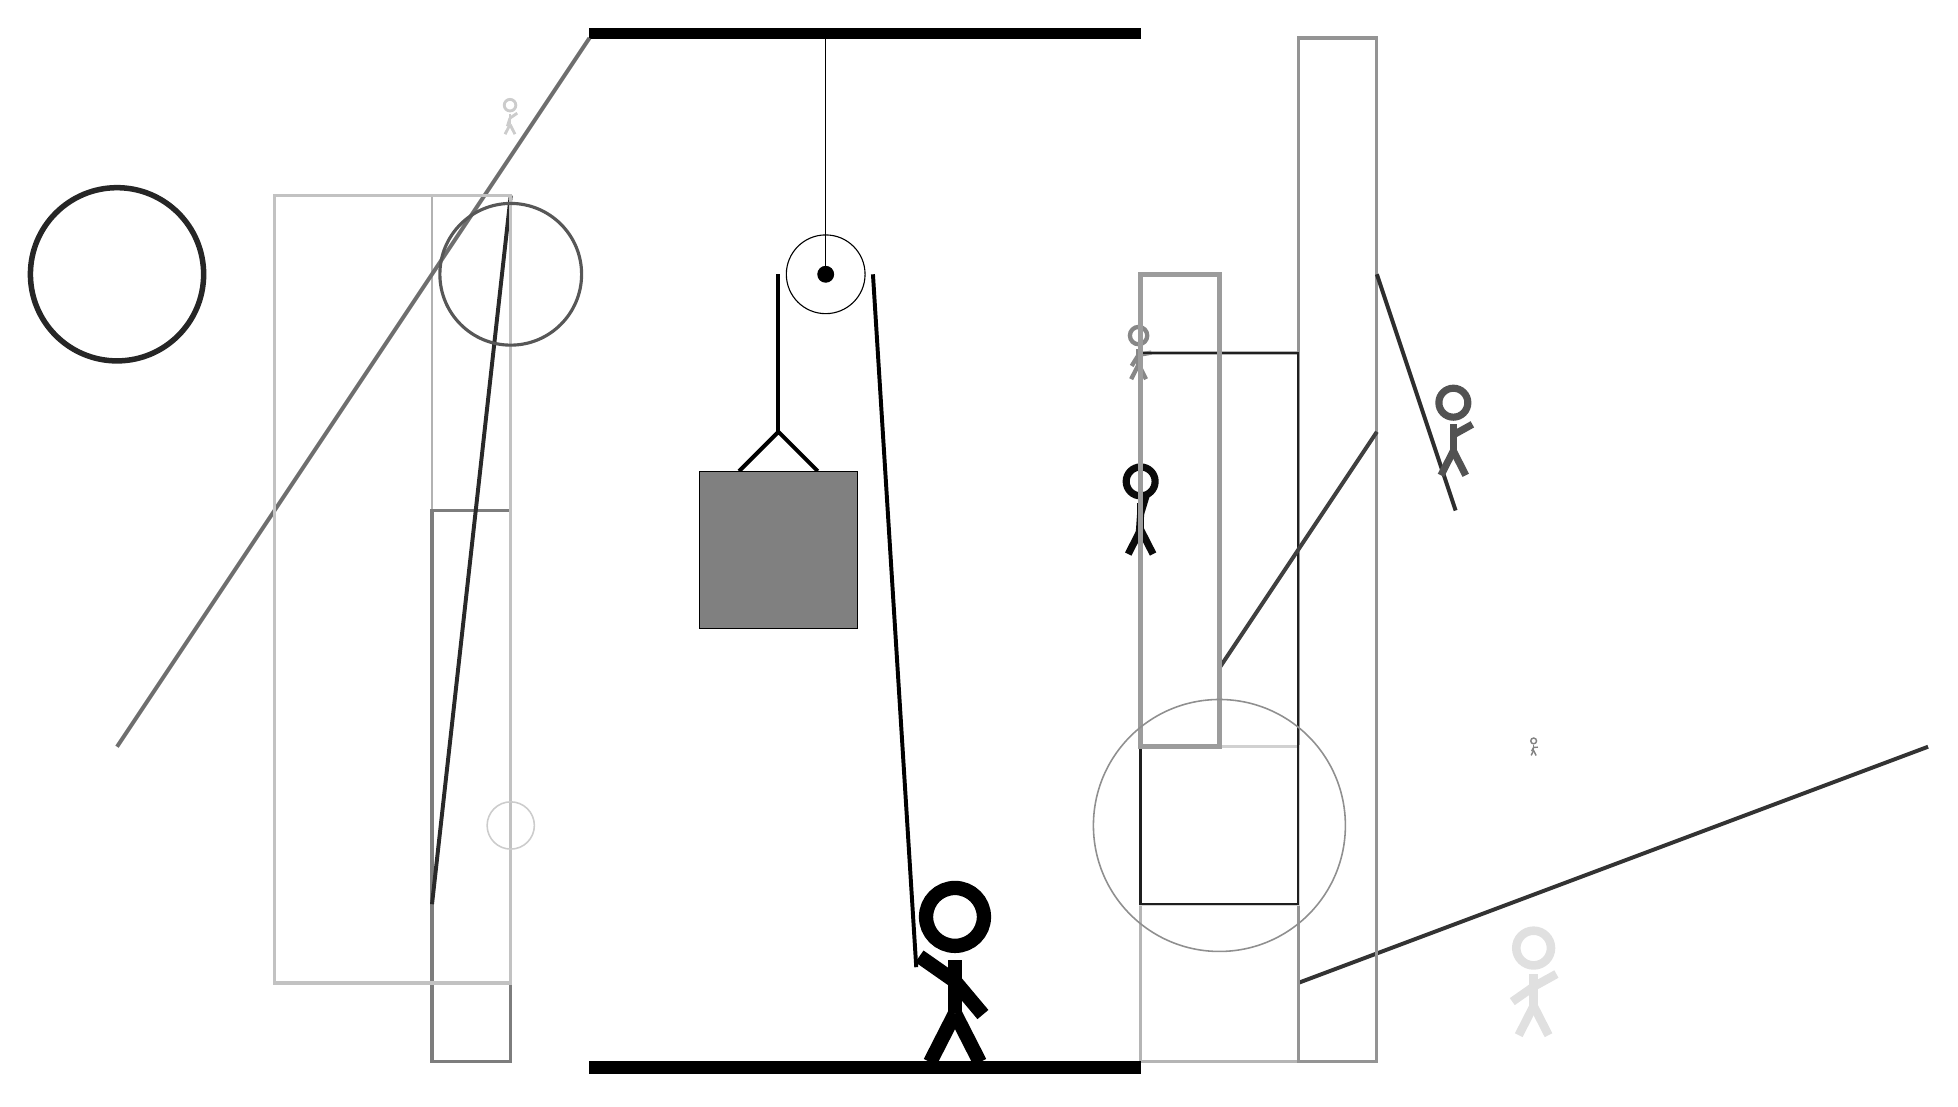
\begin{tikzpicture}
		%%%%% START %%%%%
		
		\draw[fill=black] (-2, 10) rectangle (5, 10.125);
		
		\draw[line width=0.5mm, color=black!80](7, -2) -- (15, 1);
		
		\draw[line width=0.4mm, color=black!29] (5, 6) rectangle (7, -3);
		\draw[line width=0.3mm, color=black!30] (-4, 8) rectangle (-3, -2);
		\node[line width=0.3mm, color=black!49] at (10, 1) {\Strichmaxerl[1][62][2]};
		\node[line width=0.2mm, color=black!47] at (5, 6) {\Strichmaxerl[3][58][10]};
		\draw[line width=0.4mm, color=black!51] (-3, -3) rectangle (-4, 4);
		\draw[line width=0.4mm, color=black!42] (7, -3) rectangle (8, 10);
		\node[line width=0.3mm, color=black!20] at (-3, 9) {\Strichmaxerl[2][72][34]};
		\draw[line width=0.5mm, color=black!57](-2, 10) -- (-8, 1);
		\draw[line width=0.5mm, color=black!84](-3, 8) -- (-4, -1);
		\draw[line width=0.4mm, color=black!18] (7, -1) rectangle (5, 1);
		\draw[line width=0.3mm, color=black!88] (5, 6) rectangle (7, -1);
		\draw[line width=0.4mm, color=black!24] (-3, 8) rectangle (-6, -2);
		
		\draw[line width=0.5mm, color=black!75](6, 2) -- (8, 5);
		\node[line width=0.7mm, color=black!12] at (10, -2) {\Strichmaxerl[6][35][29]};
		\draw[line width=0.5mm, color=black!82](9, 4) -- (8, 7);
		
		\node[line width=0.4mm, color=black!68] at (9, 5) {\Strichmaxerl[5][90][29]};
		\node[line width=0.3mm, color=black!96] at (5, 4) {\Strichmaxerl[5][86][73]};
		\draw[line width=0.7mm, color=black!39] (5, 1) rectangle (6, 7);
		\draw [line width=0.4mm, color=black!66](-3, 7) circle (0.9);
		\draw [line width=0.7mm, color=black!85](-8, 7) circle (1.1);
		
		\draw [line width=0.2mm, color=black!44](6, 0) circle (1.6);
		\draw [line width=0.2mm, color=black!20](-3, 0) circle (0.3);
		
		\draw (1, 7) circle (0.5);
		\draw[fill=black] (1, 7) circle (0.1);
		\draw (1, 10) -- (1, 7);
		
		\draw[line width=0.5mm] (-0.1, 4.5) -- (0.4, 5.0) -- (0.9, 4.5);
		\draw[fill=black!50] (-0.6, 4.5) rectangle (1.4, 2.5);
		
		\draw[line width=0.5mm] (0.4, 7) -- (0.4, 5.0);
		\centerarc[line width=0.5mm](1, 7)(0:180:0.6);
		\draw[line width=0.5mm](1.6, 7) -- (2.15, -1.8);
		
		\node at (2.6, -1.9) {\Strichmaxerl[10][-35][-50]};
		
		\draw[fill=black] (-2, -3) rectangle (5, -3.15);
		
		%%%%% END %%%%%
	\end{tikzpicture}
\end{document}